% Renewal oracle v2 (proposal, phase 175): heading-free edge following +
% heading re-anchoring at the wall. Compile: pdflatex renewal_oracle_v2_flow.tex
\documentclass[tikz,border=8pt]{standalone}
\usepackage{amsmath}
\usetikzlibrary{arrows.meta,positioning,fit,backgrounds,calc,shapes.geometric}

\definecolor{keep}{HTML}{E8E8E8}
\definecolor{changed}{HTML}{FCE3C2}
\definecolor{new}{HTML}{CFE3F7}
\definecolor{term}{HTML}{CDEBD3}
\definecolor{edge}{HTML}{3A3A3A}

\tikzset{
  >={Stealth[length=2.4mm]},
  every node/.style={font=\small},
  state/.style={rectangle, rounded corners=3pt, draw=edge, thick, align=center,
                minimum width=36mm, minimum height=11mm, inner sep=4pt},
  proc/.style={rectangle, draw=edge, align=center, minimum width=34mm,
               minimum height=9mm, inner sep=3pt},
  dec/.style={diamond, aspect=2.4, draw=edge, align=center, inner sep=1pt, font=\footnotesize},
  lab/.style={font=\footnotesize, fill=white, inner sep=1.5pt},
  note/.style={rectangle, draw=edge!60, dashed, align=left, font=\footnotesize,
               text width=62mm, inner sep=4pt, fill=white},
  flow/.style={->, thick, draw=edge},
}

\begin{document}
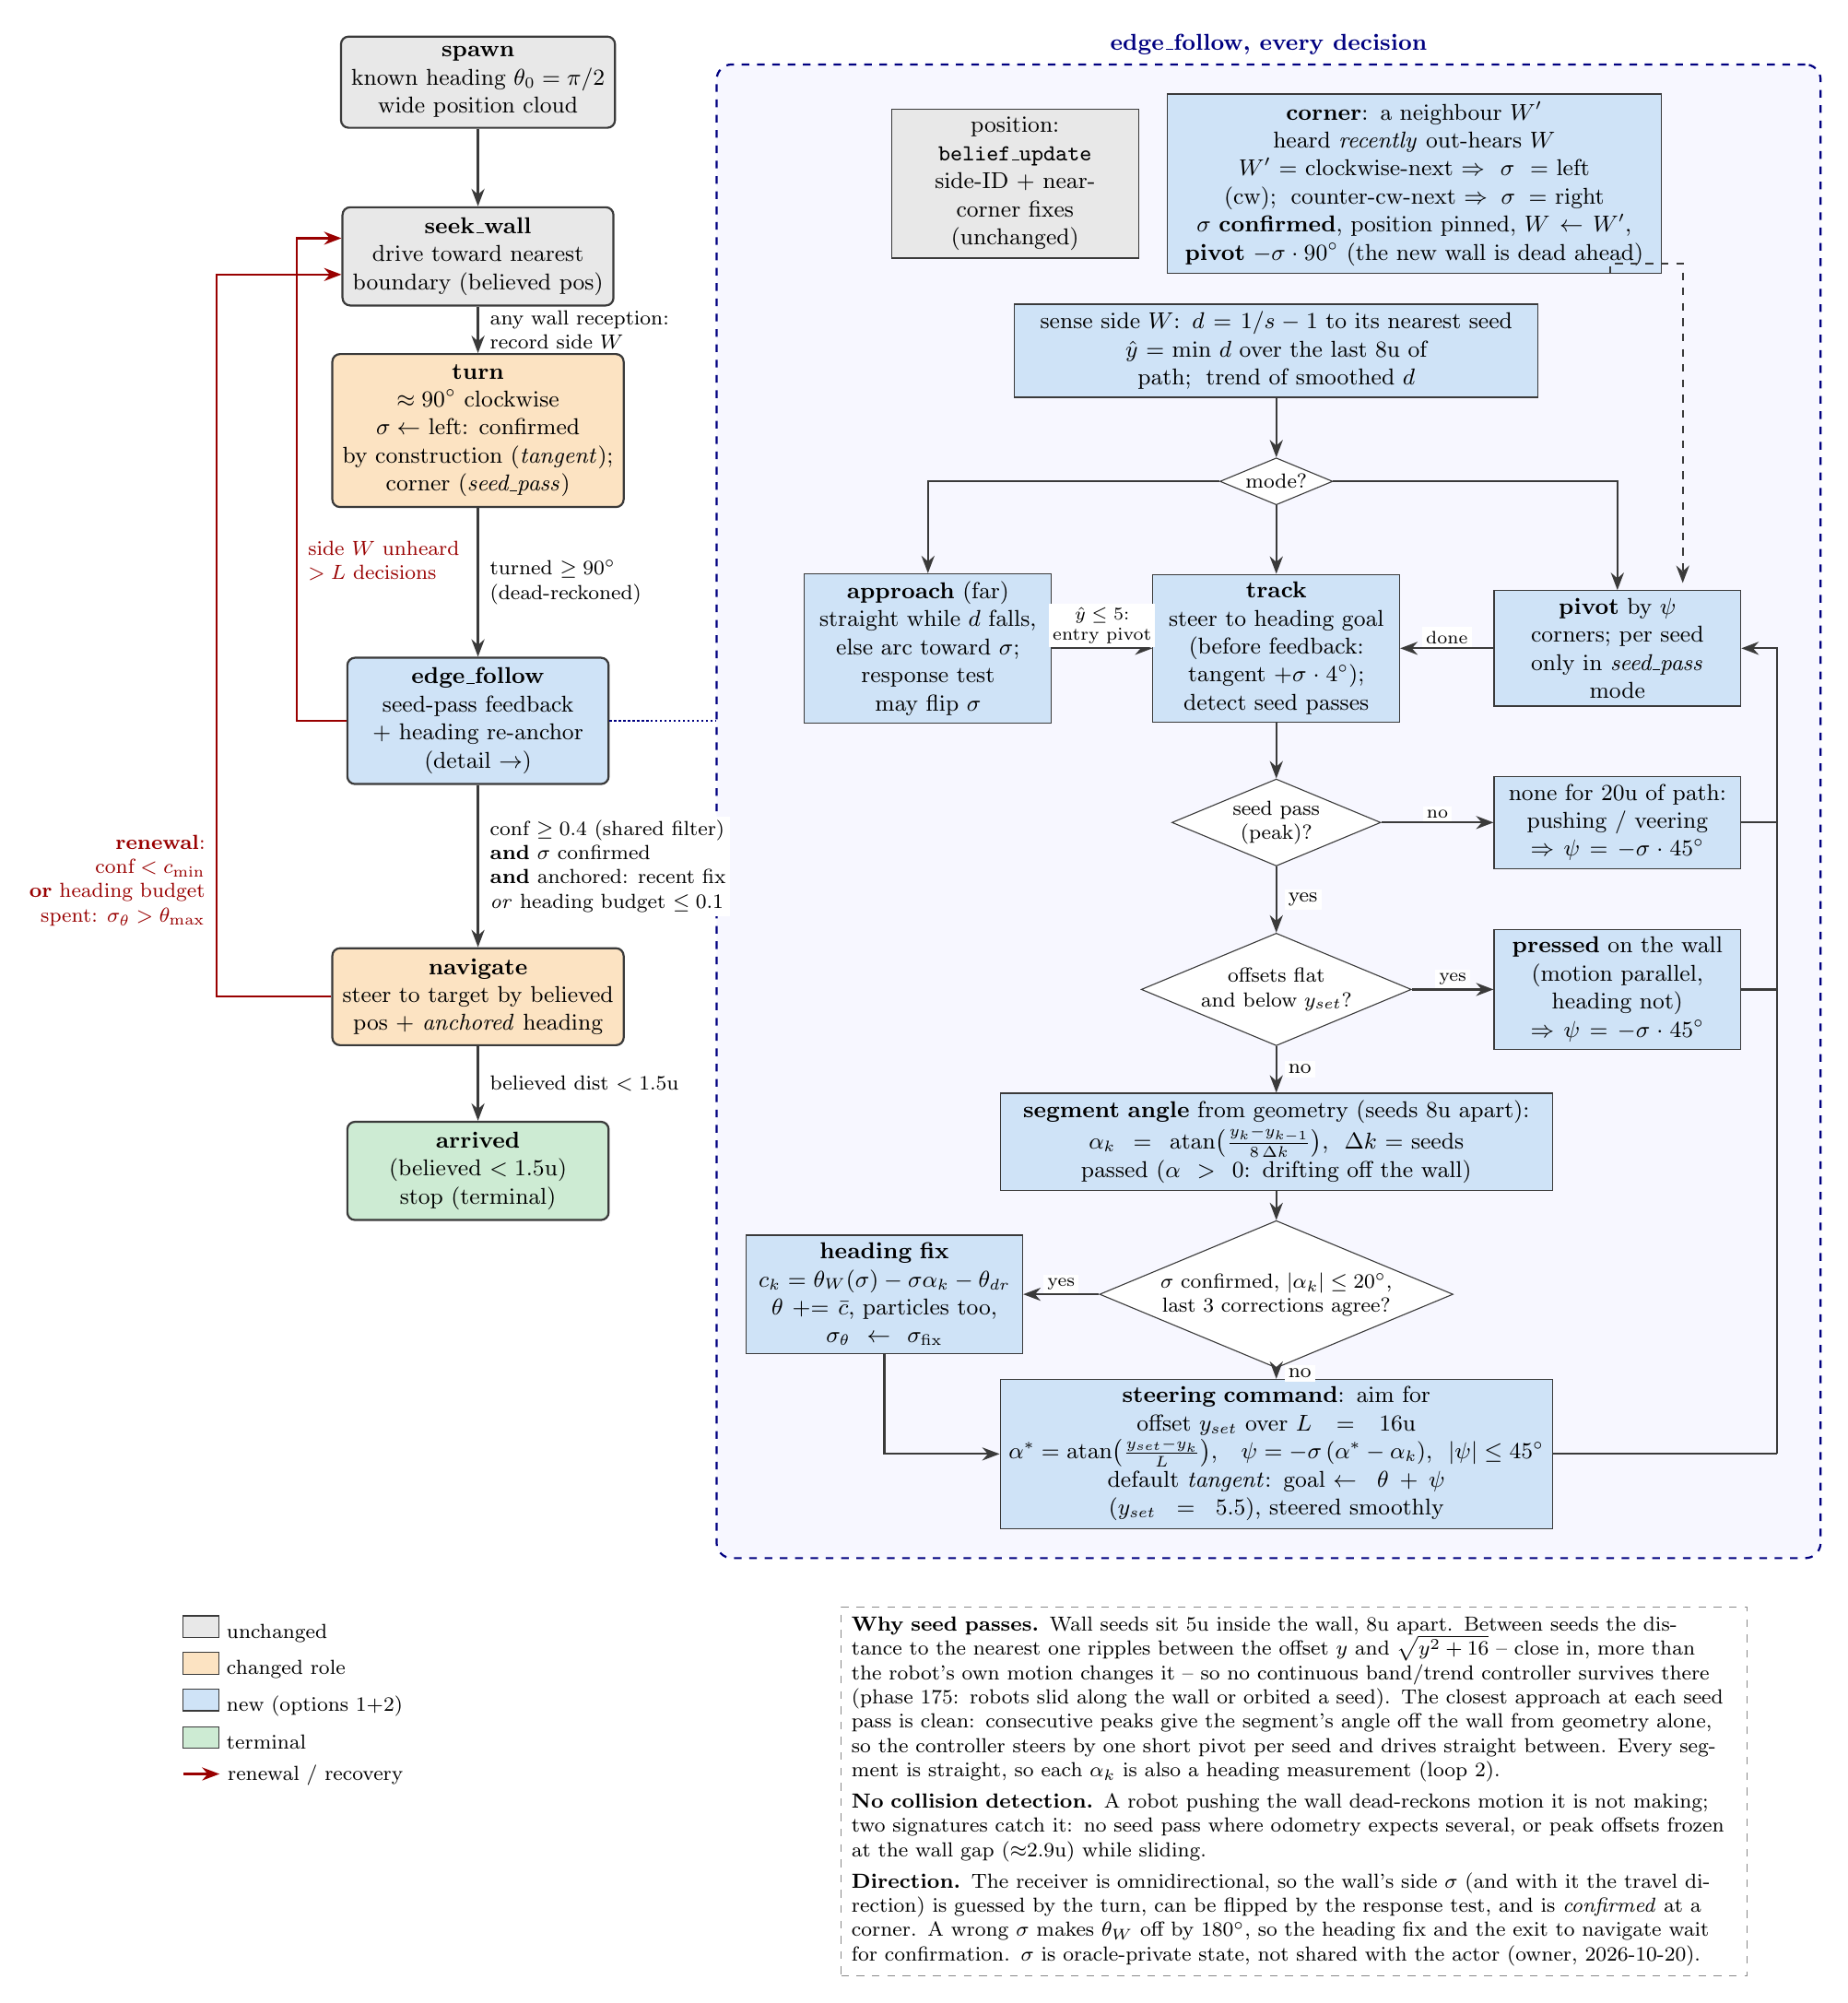
\begin{tikzpicture}[x=1cm, y=1cm]

% ------------------------------------------------------------ main column
\node[state, fill=keep] (spawn) at (0,0) {\textbf{spawn}\\ known heading $\theta_0=\pi/2$\\ wide position cloud};
\node[state, fill=keep] (seek) at (0,-2.4) {\textbf{seek\_wall}\\ drive toward nearest\\ boundary (believed pos)};
\node[state, fill=changed] (turn) at (0,-4.8) {\textbf{turn}\\ $\approx 90^\circ$ clockwise\\ $\sigma \leftarrow$ left: confirmed\\ by construction (\emph{tangent});\\ corner (\emph{seed\_pass})};
\node[state, fill=new, minimum height=17mm] (ef) at (0,-8.8)
     {\textbf{edge\_follow}\\ seed-pass feedback\\ + heading re-anchor\\ (detail $\rightarrow$)};
\node[state, fill=changed] (nav) at (0,-12.6) {\textbf{navigate}\\ steer to target by believed\\ pos + \emph{anchored} heading};
\node[state, fill=term] (arr) at (0,-15.0) {\textbf{arrived}\\ (believed $< 1.5$u)\\ stop (terminal)};

\draw[flow] (spawn) -- (seek);
\draw[flow] (seek) -- node[lab, right=1mm, align=left] {any wall reception:\\ record side $W$} (turn);
\draw[flow] (turn) -- node[lab, right=1mm, align=left] {turned $\ge 90^\circ$\\ (dead-reckoned)} (ef);
\draw[flow] (ef) -- node[lab, right=1mm, align=left]
     {conf $\ge 0.4$ (shared filter)\\ \textbf{and} $\sigma$ confirmed\\ \textbf{and} anchored: recent fix\\ \emph{or} heading budget $\le 0.1$} (nav);
\draw[flow] (nav) -- node[lab, right=1mm] {believed dist $< 1.5$u} (arr);

% lost-wall exit (inner left route)
\draw[flow, draw=red!60!black] (ef.west) -- (-2.5,-8.8) -- (-2.5,-2.15) -- (seek.west |- 0,-2.15);
\node[lab, anchor=west, align=left, text=red!60!black] at (-2.4,-6.6) {side $W$ unheard\\ $> L$ decisions};

% renewal loop (outer left route)
\draw[flow, draw=red!60!black] (nav.west) -- (-3.6,-12.6) -- (-3.6,-2.65) -- (seek.west |- 0,-2.65);
\node[lab, anchor=east, align=right, text=red!60!black] at (-3.7,-11.0)
     {\textbf{renewal}:\\ $\text{conf} < c_{\min}$\\ \textbf{or} heading budget\\ spent: $\sigma_\theta > \theta_{\max}$};

% ------------------------------------------------------------ edge_follow detail
\node[proc, fill=keep, text width=31mm] (pos) at (7.4,-1.4)
     {position: \texttt{belief\_update}\\ side-ID + near-corner fixes\\ (unchanged)};
\node[proc, fill=new, text width=66mm] (corner) at (12.9,-1.4)
     {\textbf{corner}: a neighbour $W'$ heard \emph{recently} out-hears $W$\\
      $W'$ = clockwise-next $\Rightarrow \sigma=$ left (cw);\; counter-cw-next $\Rightarrow \sigma=$ right\\
      $\sigma$ \textbf{confirmed}, position pinned, $W \leftarrow W'$,\\
      \textbf{pivot} $-\sigma\cdot 90^\circ$ (the new wall is dead ahead)};
\node[proc, fill=new, text width=70mm] (sense) at (11,-3.7)
     {sense side $W$: $d = 1/s - 1$ to its nearest seed\\
      $\hat y$ = min $d$ over the last 8u of path;\; trend of smoothed $d$};
\node[dec, fill=white] (mode) at (11,-5.5) {mode?};

\node[proc, fill=new, text width=30mm] (appr) at (6.2,-7.8)
     {\textbf{approach} (far)\\ straight while $d$ falls,\\ else arc toward $\sigma$;\\ response test may flip $\sigma$};
\node[proc, fill=new, text width=30mm] (track) at (11,-7.8)
     {\textbf{track}\\ steer to heading goal\\ (before feedback:\\ tangent $+\sigma\cdot4^\circ$);\\ detect seed passes};
\node[proc, fill=new, text width=28mm] (pivot) at (15.7,-7.8)
     {\textbf{pivot} by $\psi$\\ corners; per seed\\ only in \emph{seed\_pass}\\ mode};
\draw[flow] (sense) -- (mode);
\draw[flow] (mode) -| (appr);
\draw[flow] (mode) -- (track);
\draw[flow] (mode) -| (pivot);
\draw[flow] (appr.east) -- node[lab, above, font=\scriptsize, align=center] {$\hat y \le 5$:\\ entry pivot} (track.west);
\draw[flow] (pivot.west) -- node[lab, above, font=\scriptsize] {done} (track.east);

\node[dec, fill=white] (peak) at (11,-10.2) {seed pass\\ (peak)?};
\node[proc, fill=new, text width=30mm] (nopeak) at (15.7,-10.2)
     {none for 20u of path:\\ pushing / veering\\ $\Rightarrow \psi = -\sigma\cdot 45^\circ$};
\node[dec, fill=white] (press) at (11,-12.5) {offsets flat\\ and below $y_{set}$?};
\node[proc, fill=new, text width=30mm] (pressed) at (15.7,-12.5)
     {\textbf{pressed} on the wall\\ (motion parallel,\\ heading not)\\ $\Rightarrow \psi = -\sigma\cdot 45^\circ$};
\node[proc, fill=new, text width=74mm] (angle) at (11,-14.6)
     {\textbf{segment angle} from geometry (seeds 8u apart):\\
      $\alpha_k = \operatorname{atan}\!\big(\tfrac{y_k - y_{k-1}}{8\,\Delta k}\big)$, \ $\Delta k$ = seeds passed ($\alpha>0$: drifting off the wall)};
\node[dec, fill=white] (fitd) at (11,-16.7) {$\sigma$ confirmed, $|\alpha_k|\le 20^\circ$,\\ last 3 corrections agree?};
\node[proc, fill=new, text width=36mm] (fix) at (5.6,-16.7)
     {\textbf{heading fix}\\ $c_k = \theta_W(\sigma) - \sigma\alpha_k - \theta_{dr}$\\
      $\theta \mathrel{+}= \bar c$, particles too,\\ $\sigma_\theta \leftarrow \sigma_{\text{fix}}$};
\node[proc, fill=new, text width=74mm] (cmd) at (11,-18.9)
     {\textbf{steering command}: aim for offset $y_{set}$ over $L=16$u\\
      $\alpha^\ast = \operatorname{atan}\!\big(\tfrac{y_{set}-y_k}{L}\big)$,\quad $\psi = -\sigma\,(\alpha^\ast - \alpha_k)$, \ $|\psi|\le 45^\circ$\\
      default \emph{tangent}: goal $\leftarrow \theta + \psi$ ($y_{set}=5.5$), steered smoothly};

\draw[flow] (track) -- (peak);
\draw[flow] (peak) -- node[lab, right=1mm] {yes} (press);
\draw[flow] (peak) -- node[lab, above, font=\scriptsize] {no} (nopeak);
\draw[flow] (press) -- node[lab, right=1mm] {no} (angle);
\draw[flow] (press) -- node[lab, above, font=\scriptsize] {yes} (pressed);
\draw[flow] (angle) -- (fitd);
\draw[flow] (fitd) -- node[lab, above, font=\scriptsize] {yes} (fix);
\draw[flow] (fitd) -- node[lab, right=1mm] {no} (cmd);
\draw[flow] (fix.south) |- (cmd.west);
% the pivot bus: every pivot request feeds the pivot mode
\draw[thick, draw=edge] (nopeak.east) -- (17.9,-10.2);
\draw[thick, draw=edge] (pressed.east) -- (17.9,-12.5);
\draw[thick, draw=edge] (cmd.east) -- (17.9,-18.9);
\draw[flow] (17.9,-18.9) -- (17.9,-7.8) -- (pivot.east);
\draw[flow, dashed] (corner.south -| 15.6,0) -- (15.6,-2.5) -| (16.6,-6.9);

\coordinate (boxedge) at (18.1,-18.9);
\begin{scope}[on background layer]
  \node[draw=blue!50!black, thick, dashed, rounded corners=6pt, fill=blue!3,
        fit=(pos)(corner)(sense)(appr)(pivot)(fix)(cmd)(boxedge), inner sep=4mm,
        label={[font=\small\bfseries, text=blue!50!black]above:edge\_follow, every decision}] (box) {};
\end{scope}
\draw[thick, densely dotted, draw=blue!50!black] (ef.east) -- (box.west |- ef.east);

% ------------------------------------------------------------ notes + legend
\node[note, anchor=north west, text width=122mm] (notes) at (5.0,-21.0)
     {\textbf{Why seed passes.} Wall seeds sit 5u inside the wall, 8u apart. Between seeds the
      distance to the nearest one ripples between the offset $y$ and $\sqrt{y^2+16}$ -- close in, more
      than the robot's own motion changes it -- so no continuous band/trend controller survives
      there (phase 175: robots slid along the wall or orbited a seed). The closest approach at each
      seed pass is clean: consecutive peaks give the segment's angle off the wall from geometry
      alone, so the controller steers by one short pivot per seed and drives straight between.
      Every segment is straight, so each $\alpha_k$ is also a heading measurement (loop 2).\\[1mm]
      \textbf{No collision detection.} A robot pushing the wall dead-reckons motion it is not making;
      two signatures catch it: no seed pass where odometry expects several, or peak offsets frozen
      at the wall gap ($\approx$2.9u) while sliding.\\[1mm]
      \textbf{Direction.} The receiver is omnidirectional, so the wall's side $\sigma$ (and with it the
      travel direction) is guessed by the turn, can be flipped by the response test, and is
      \emph{confirmed} at a corner. A wrong $\sigma$ makes $\theta_W$ off by $180^\circ$, so the heading fix
      and the exit to navigate wait for confirmation. $\sigma$ is oracle-private state, not shared
      with the actor (owner, 2026-10-20).};

\node[anchor=north west, align=left, font=\footnotesize] at (-4.2,-21.0) {%
  \tikz\node[fill=keep,draw=edge,minimum width=5mm,minimum height=3mm]{}; unchanged\\[1mm]
  \tikz\node[fill=changed,draw=edge,minimum width=5mm,minimum height=3mm]{}; changed role\\[1mm]
  \tikz\node[fill=new,draw=edge,minimum width=5mm,minimum height=3mm]{}; new (options 1+2)\\[1mm]
  \tikz\node[fill=term,draw=edge,minimum width=5mm,minimum height=3mm]{}; terminal\\[1mm]
  \tikz\draw[->,thick,red!60!black](0,0)--(5mm,0); renewal / recovery};

\end{tikzpicture}
\end{document}
